\chapter{3D Buckled Mesostructures}
\label{ch:mesostructures}
\graphicspath{{mesostructures/fig/}}

This chapter is based upon the joint work: Y. Li, S. J. Avis, J. Chen, G. Wu, T. Zhang, H. Kusumaatmaja, and X. Wang, ``Reconfiguration of multistable 3D ferromagnetic mesostructures guided by energy landscape surveys'', \emph{Extreme Mech. Lett.}, 48, 101428 (2021).

In particular, the experimental ferromagnetic structures are the work of Y. Li, while the simulations and energy landscape analysis are my own work.


\section{Introduction}

Reconfigurable three-dimensional structures that can actively change their geometries and thereby their functionalities upon external stimuli (like mechanical forces, magnetic fields, hydration, and temperature) \cite{Overvelde2017,Filipov2015,Wehner2016,Kim2018,Gladman2016,Xie2010} are promising for a diverse range of applications including deployable solar panels \cite{Thesiya2015}, metamaterials \cite{Fu2011,Wang2017,Lee2020}, phononics \cite{Babaee2016,Deng2020}, biomedical devices \cite{Damdam2019,Anderson2017}, robotics \cite{Plitea2013,Tang2019,Gorissen2020}, metasurfaces \cite{Liu2019a,Wang2016}, and many others.
The design of reconfigurable structures usually relies on structural instabilities \cite{Chen2012,Jiang2019,Zareei2020}, stimuli-responsive constituent materials (like swellable gels, shape memory polymers and magnetic materials) \cite{Gladman2016,Lendlein2005,Kim2012,Novelino2020,Liu2019b}, or their heterogeneous combinations \cite{Ding2017}.

As discussed in \cref{sec:es-mesostructures}, structural instabilities of simple 2D patterns under compression have been exploited to produce 3D buckled mesostructures, and can be used to realise a diverse range of complex 3D functional architectures and electronics \cite{Xu2015,Zhang2015,Wang2019a,Jang2017,Lee2018a}.
Through elastically deforming the assembly platform in different time sequences (i.e., loading-path control), the 3D structures have been shown to morph into different shapes \cite{Fu2018,Pang2020}.
In addition to mechanical deformation, reconfigurable structures can also be realised through active materials including ferromagnetic composites \cite{Kim2018,Kim2019,Hu2018,Boncheva2005}, hydrogels \cite{Gladman2016}, shape memory polymers (SMPs) \cite{Xie2010,Wang2019a}, liquid crystal elastomers (LCEs) \cite{White2015}, and electrochemically active materials \cite{Xia2019}, which can change their shape upon external stimuli.

In recent years, an emerging attractive strategy to realise robust reconfigurable structures is to encode multiple stable states by design that do not require persistent external stimuli \cite{Song2019,Yang2019,ODonnell2020,Li2020}.
Each of these stable states is a local minimum in a complex energy landscape, and therefore only a temporary external stimulus is needed to guide the structure from one state to another, after which it will remain in that state.

Despite intensive studies, a number of critical challenges remain, especially when asymmetric and complicated modes are involved in the architectural reconfiguration.
The first challenge is associated with the presence of multiple local minimum configurations, which could affect the stability of the targeted stable state under perturbations (e.g., environmental noises) or trap the structure in an intermediate state during the process of reconfiguration.
For example, it is recently recognised by researchers that hidden local minimum configurations can destroy the designed pathway of deploying origami structures \cite{Na2015,Silverberg2015}.
Thus, it is crucial to provide means of manipulating the energy well depth of targeted configurations and eliminating unfavorable local minima in the design of reconfigurable structures.

The second challenge stems from the complexity of the transition paths from one local minimum state to another, especially when the two states are separated by other stable and transition states \cite{Groh2019,Virot2017,Marthelot2017,Medina2020,Panter2019}.
A recent work \cite{Panter2019} shows that the transition from a uniformly deformed cylindrical shell to a 9-dimple buckled pattern needs to pass 7 local minimum configurations, which cannot be achieved by directly applying local probes to the shell.
Complicated transition paths among local minima are also found in mechanical metamaterials, which further provides new design parameters to program the deformed configurations of the structures \cite{Medina2020}.

Finally, it is also very challenging to realise remote, locally controlled, and rapid reconfiguration of the deformed, highly nonlinear structures \cite{Fu2018,Luo2019}.
These challenges call for a new means of systematically surveying the energy landscapes of the multistable structures to probe and tailor the energy barrier height among different local minima.

In this chapter, we develop a set of strategies to address these challenges and to guide the design of ferromagnetic 3D mesostructures, which are developed by our collaborators.
The use of ferromagnetic materials enables remote and rapid reconfiguration among different stable states via a portable magnet, eliminating the need for mechanical stages to apply controlled, global deformations to the substrate, as used in previous works \cite{Fu2018,Pang2020}.
Thus providing opportunities for remote, tetherless shape morphing, which is advantageous for many applications, especially those that require shape morphing in enclosed or delicate environments such as robotics and biomedical devices.

Theoretically, we employ a discrete shell model \cite{Seung1988,Grinspun2003} and path-finding algorithms \cite{Panter2019,E2007} to conduct fundamental studies on the complicated energy landscapes of the 3D ferromagnetic structures.
We construct design phase diagrams showing how the available stable states sensitively depend on the essential material and geometrical parameters of the elastic structures.
Furthermore, the minimum energy reconfiguration paths between the stable states and their energy barriers are identified using a combination of our developed BITSS method and the string method \cite{E2007}.
A salient advantage of our approach is that it allows the computation of reconfiguration paths following the minimum energy pathways (MEPs) systematically without the need to assume a predefined path for the structural transformation.

Our methodology is versatile and is applied to design and realise reconfigurable structures with a wide range of geometries, including ribbons and structures that resemble tables, baskets, flowers, boxes, single and double beams.
In all cases, the theoretically predicted and experimentally realised shapes and reconfiguration paths are in excellent agreement.
We also demonstrate reconfiguration of structures fabricated from non-active materials that are locally patterned with ferromagnetic films, which significantly expands the design space and material libraries for reconfigurable structures.

% Based upon these results, we highlight some proof- applications that have created by our experimental collaborators.
To further demonstrate the versatility of these reconfigurable 3D ferromagnetic structures, we highlight a number of applications that have been created by our experimental collaborators.
This includes a reconfigurable light emitting system, which illustrates the capacity to integrate other functional components into the 3D structures.
Finally, magnetically actuated particle delivery is shown, which utilises the different reconfigurational modes of a table structure.



\section{Results}

\subsection{Phase diagram of stable states for a table structure}

\Cref{fig:ms-1}(a) schematically illustrates the assembly process of a 3D structure from ferromagnetic composite thin films via compressive buckling, and the architectural reconfiguration of the structure via magnetic actuation.
The ferromagnetic composite is prepared by homogeneously embedding hard NdFeB (neodymium-iron-boron) microparticles into a soft elastomer, polydimethylsiloxane (PDMS).
These are then patterned into 2D layouts using a CO2 laser, followed by their magnetization using impulse magnetic fields (about 2.7 T).
They are then attached to a prestretched elastomeric substrate using a very thin layer of superglue to generate strong bonding at select location on the 2D patterns.
Releasing the prestrain in the substrate leads to compressive forces on the 2D ferromagnetic pattern at the bonding sites and geometrically transforms the pattern into a 3D structure.
We define the 2D layout to lie on the $x$-$y$ plane so that its normal vector is in the $z$ direction.

\begin{figure}[H]
  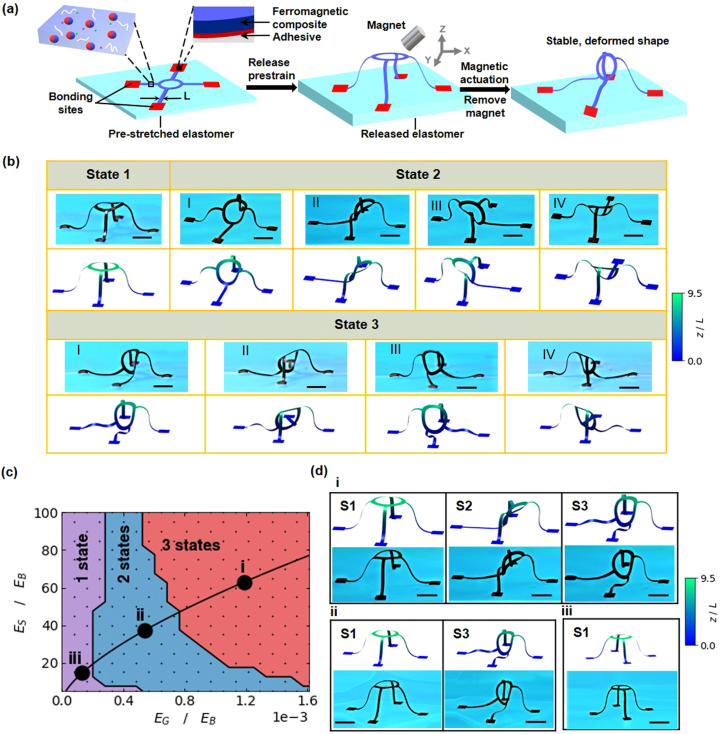
\includegraphics[width=\textwidth]{figure1.jpg}
  \caption{
    Multistability of magnetically reconfigurable 3D structures.
    (a) Schematic illustrating the assembly and reconfiguration of 3D ferromagnetic structures.
    (b) Experimental and computational results of multistable states in a 3D table structure.
    (c) Design phase diagram showing the number of distinct stable states based on the energy scales of the table structure.
        Representative examples in each regime with different values of $L$ are marked.
    (d) Experimental and computational results of the distinct stable states for the three representative examples marked in (c).
        S1-S3 refer to state 1-3, respectively.
    Scale bars, \SI{1}{\centi\meter}.
  }
  \label{fig:ms-1}
\end{figure}

To efficiently explore the possible stable states existing in the table structure, we simulate the structure using a simple discrete shell model.
The surface is discretised using a Delaunay triangulation \cite{Rebay1993}, with a target mesh size of a tenth of the ribbon width, and then the energy is calculated using the bar-and-hinge model discussed in \cref{sec:ell-bah}.
In these simulations, we assign the Young’s modulus of the ferromagnetic film to be $Y=\SI{1.4}{\mega\pascal}$ \cite{Kim2019} and use a thickness, $t=\SI{150}{\micro\meter}$.
The gravitational force is also included by setting the film density to its measured experimental value of $\rho = \SI{2.59}{\gram\per\centi\meter\cubed}$.
These parameters, and others used in this chapter, are listed in \cref{tab:or-params}.
Finally, we model the repulsive substrate interaction using a Lennard-Jones 3-9 potential with the attractive region removed.
Consequently, the model does not take into consideration the effect of adhesion which may become significant at small scales.

The stable states are obtained by minimizing the structures energy using the L-BFGS algorithm \cite{Nocedal1980,Liu1989}, which is highly efficient for minimization involving a large number of degrees of freedom.
The structures are buckled by steadily moving the binding sites from their positions in the flat precursor to their final positions over the first \num{10000} iterations.
While this buckling is taking place, the structure is split into a number of different regions and each is given a random force to enable the structure to take different configurations.
This process is repeated several hundreds of times to identify the different local minima in the energy landscape.

\Cref{fig:ms-1}(b) presents experimental and corresponding computational results of a 3D ferromagnetic table structure and its multiple stable states.
The table structure is oriented in a way such that gravity is perpendicular to the substrate (in the negative $z$ direction), which is the case for most of the structures in this study unless specified otherwise.

Three distinct states (state 1-3) with a total of nine configurations are discovered.
Magnetically deforming the assembled table structure via a portable disk magnet, with one leg becoming flat while the other three legs remain buckled, rapidly reconfigures the table structure from state 1 into a distinct stable state 2, with four different orientational configurations (state 2: shape I-IV).
Further magnetic actuation induces an additional leg of the table structure to become flat and results in the transition from state 2 into another stable state with four different orientations (state 3: shape I-IV).
In addition, unlike previously reported reconfigurable 3D structures that rely on persistent external stimuli to maintain their deformed shapes \cite{Kim2018,Gladman2016,White2015,Hajiesmaili2019}, the deformed configurations of the table structure shown here can well maintain their shapes after the applied magnetic field is removed, as they are locally stable configurations.
Computational modelling results of the configurations for the stable states and their different orientations via the discrete shell model are highly consistent with experiments, with the colour in the results denoting the displacement of the structure along the $z$ direction.

Using the combined experimental and computational strategy, we further study the effect of essential geometry and material properties on the entire spectrum of existing stable states, yielding the design phase diagram shown in \cref{fig:ms-1}(c).
The diagram illustrates the total number of stable states according to two dimensionless parameters that are determined from the ratios between three relevant energy scales – gravitational ($E_G$), stretching ($E_S$), and bending ($E_B$).
These energy scales can be expressed in terms of the material and geometric parameters of the 3D structure:
\begin{equation}
  E_G = \rho g L^3 t, \qquad E_S = Y L^2 t, \qquad E_B = \frac{Yt^3}{1-\nu^2},
\end{equation}
where $\rho$ is the material density, $Y$ is the Young’s modulus, $\nu$ is the Poisson ratio, $t$ is the film thickness, and $L$ represents the in-plane size of the structure (the width of table legs is used for this study).
The cubic term of $L$ in $E_G$ comes from the fact that the volume of the structure scales with $L^2$ and the displacement in the direction of gravity is proportional to $L$.

Three regimes in terms of the number of existing stable states can be identified in \cref{fig:ms-1}(c): (i) 3 distinct stable states, (ii) 2 distinct stable states, and (iii) 1 distinct stable state, which are controlled by two dimensionless variables $E_S/E_B = L^2(1-\nu^2)/t^2$ and $E_G/E_B = \rho g L^3 (1-\nu^2) / Yt^2$.
The variable $E_S/E_B$ characterises the bendability of the structure, with a larger value indicating that it is easier to generate bending deformation.
$E_G/E_B$ describes the competition between the gravitational and bending energies.
When $E_S/E_B$ and $E_G/E_B$ are relatively large, three distinct stable states as shown in \cref{fig:ms-1}(b) exist in regime i, with states 2 and 3 having 4 different orientations.
As the two dimensionless variables decrease, state 2 becomes unstable, resulting in two distinct stable states (states 1 and 3) for regime ii.
When $E_G/E_B$ is further reduced to an even smaller value, only the buckled-up state (state 1) is stable in regime iii.

To validate the phase diagram experimentally, we fabricate 3D ferromagnetic structures of the same film thickness ($t$) and material properties ($\rho$, $Y$, and $\nu$) but of different sizes ($L$), and magnetically reconfigure them into their multistable states.
\Cref{fig:ms-1}(d) (i-iii) demonstrates the number and configurations of the stable states for structures with $L = \SI{1.04}{\milli\meter}$, \SI{0.8}{\milli\meter}, and \SI{0.5}{\milli\meter}, respectively, which agree well with the prediction of the design phase diagram.
Please note that the overall in-plane dimensions of the structures are scaled proportionally with $L$ as it varies.

The diagram provides very important guidelines for achieving a well-controlled number of stable states or for removing undesired stable states in various applications by tuning the geometry and material properties.
For instance, if state 2 is undesired, the structure can be designed with $E_S/E_B$ and $E_G/E_B$ falling within regime ii, where only states 1 and 3 are stable.


\subsection{Reconfiguration pathways of a table structure}

Identifying the optimal transition pathways between the stable states of a 3D structure is critical for well-controlled, energy-efficient reconfigurations.
By using the table structure as an example, we further examine its energy landscape to identify the minimum energy pathways (MEPs) between metastable states, in which the maximum energy along the path occurs at a saddle point (the transition state).
However, the non-linear reconfigurations of the structure can thwart standard pathway methods unless they are initialised close to the correct path, and the large number of degrees of freedom used to model the structure can make the problem computationally intractable.
Instead, to locate the pathway efficiently, a combination of methods are used.
First, the transition state is located using the BITSS method, which does not require an initial pathway guess.
By minimising downhill from either side of the transition state with L-BFGS a pathway is generated, which is then refined using the string method (introduced in \cref{sec:lm-string}).

Our approach allows automatic and systematic computation of reconfiguration paths following the MEPs without the need to assume the pathways along which the structure morphs.
This is useful because the energy-efficient reconfiguration paths can be highly complex for 3D elastic structures, and it is not always possible to prescribe an expected pathway a priori, as typically adopted in previous works where energy barriers are calculated \cite{Fang2017,Fu2018,Virot2017,Shang2018}.

As shown in \cref{fig:ms-2}(a), we find the transition pathways to progress from state 3 to state 1 of the table structure can be broadly grouped into three regions: (I) two paths, 1 and 2, exist (red region); (II) two paths, 1 and 2*, exist (orange region); (III) only path 1 exists (yellow region).
The distinction between paths 2 and 2* is that the intermediate state 2 is no longer stable on the latter.
For illustration, we construct the design diagram by varying the in-plane size of the structures ($L$), while keeping their material properties ($\rho$, $Y$, and $\nu$) and film thickness ($t=\SI{125}{\micro\meter}$) constant.
The marked red and blue points correspond to those in the 3-state and 2-state regimes identified in the design diagram in \cref{fig:ms-1}(c), respectively.

For $L > \SI{0.89}{\milli\meter}$ (region I), two independent minimum energy pathways are found and illustrated in \cref{fig:ms-2}(b) for a representative table structure with $L = \SI{1.04}{\milli\meter}$.
The first (path 1) is a direct pathway with energy barrier $\upDelta E_1$, and the second (path 2), a path that passes through state 2 as an intermediary, with energy barriers $\upDelta E_2$ between states 3 and 2 and $\upDelta E_3$ between states 2 and 1.

\begin{figure}[H]
  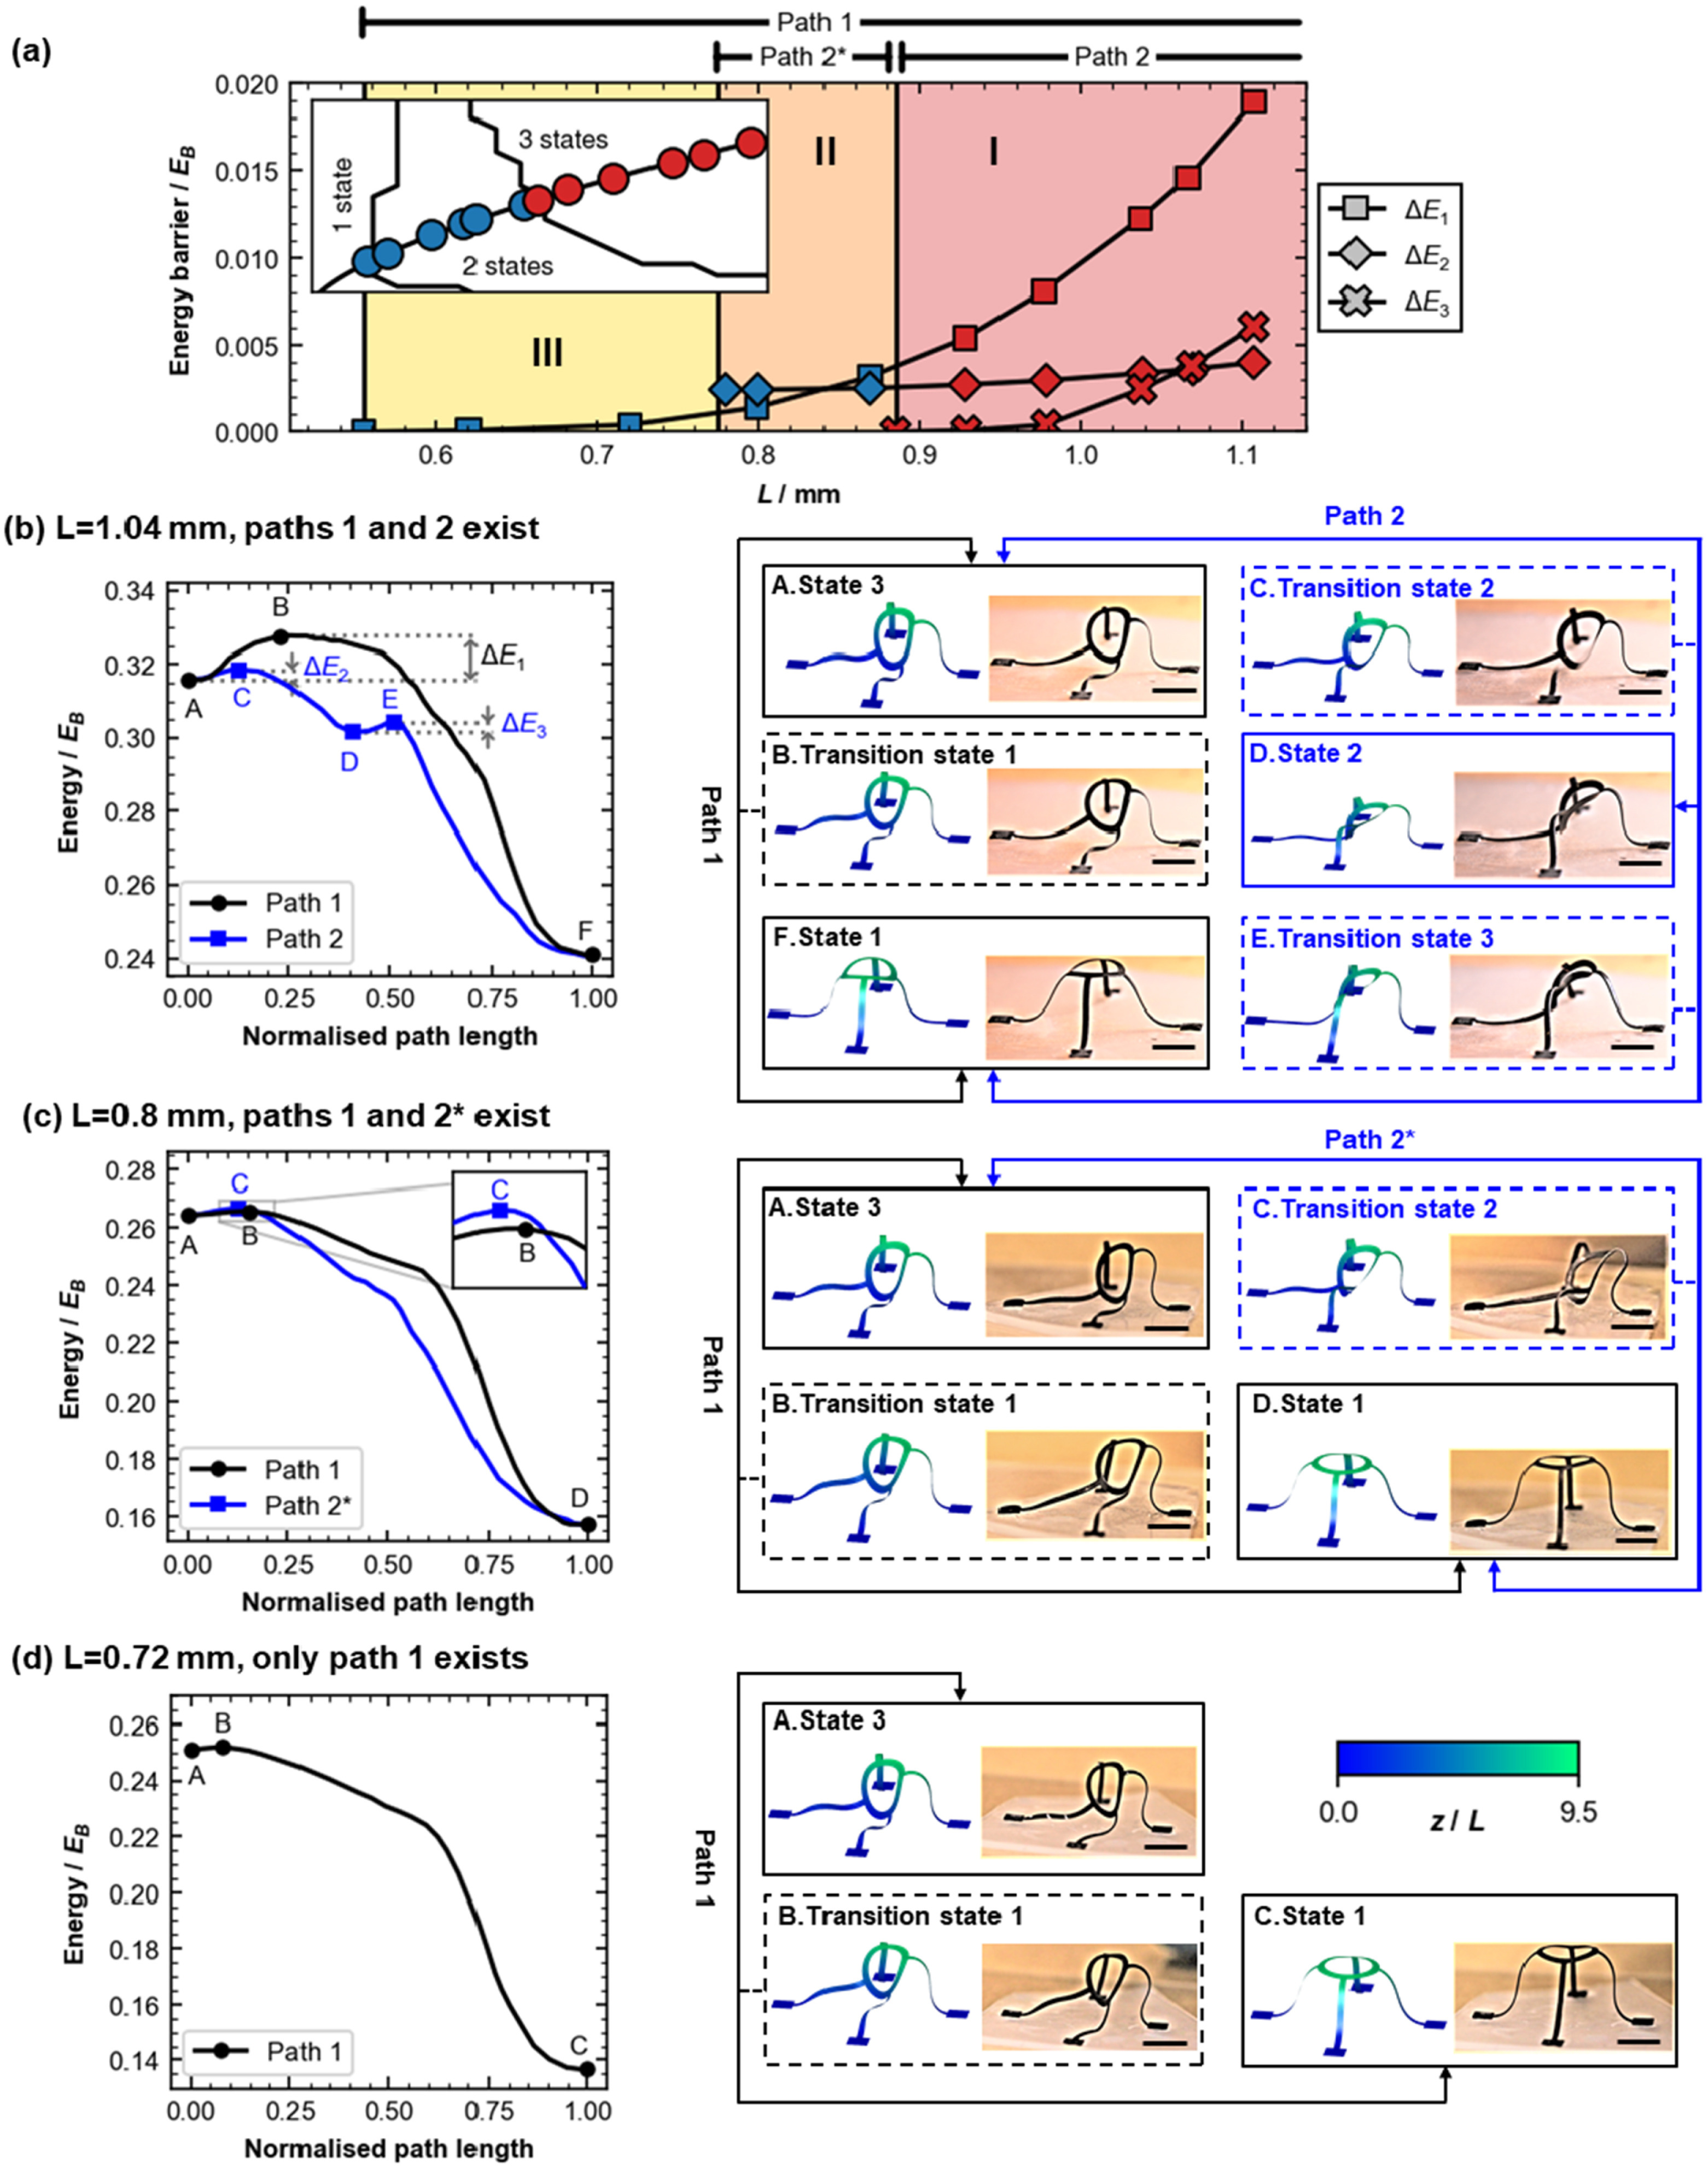
\includegraphics[width=\textwidth]{figure2.jpg}
  \caption{
    Energy barriers and reconfiguration pathways.
    (a) Variation of the energy barriers against $L$.
        Three regions (I-III) with different available pathways are highlighted.
        Inset: The locations within the design phase diagram.
    (b-d) Energy profiles and snapshots of stable and transition states for the pathways from state 3 to 1 with three values of $L$:
          (b) \SI{1.04}{\milli\meter}, (c) \SI{0.8}{\milli\meter}, and (d) \SI{0.72}{\milli\meter}.
          The energies are normalised by the bending energy.
          The definitions of the three energy barriers ($\upDelta E_1$, $\upDelta E_2$, $\upDelta E_3$) are shown in (b).
    Scale bars, \SI{1}{\centi\meter}.
  }
  \label{fig:ms-2}
\end{figure}

Snapshots of configurations along the pathways are captured in simulations and magnetic reconfiguration experiments and are shown in \cref{fig:ms-2}(b), with the complete structural transformation process and corresponding energy profiles simultaneously demonstrated in \cref{vid:pathA1,vid:pathA2}.

The energy barriers of the pathways demonstrate both the stability of the states and the ease of transitioning between them.
For example, the energy barrier to progress from state 3 to state 1 is much smaller than that from the inverse direction, thereby making state 1 more stable.
Comparing paths 1 and 2 also suggests that a smaller input energy is needed when reconfiguring the table structure along path 2 (passing two saddle points) than that along path 1.
However, the finite energy barrier $\upDelta E_3$ also indicates that the transition can be potentially trapped in state 2 if insufficient external energy is provided for reconfiguration.
In addition, reconfiguration along path 2 requires more efforts in manipulating the direction and the strength of external magnetic forces, compared to the direct pathway following path 1.

These complexities clearly show the importance of harnessing the energy landscape analysis for guiding the choice of transition paths based on specific applications and the nature of available external magnetic fields (or other external stimuli).
In addition, it is also worth noting that the pathways observed in experiments, where a portable magnet is utilised to reconfigure the structure from state 3 to state 1, are highly consistent with those from simulations, which indicates the high fidelity and reliability of the approach used in this study.
Moreover, the experimental reconfigurations can be completed within a few seconds (\cref{vid:pathA1,vid:pathA2}).
Such fast and remotely controlled transitions are desired for numerous applications, such as in soft robotics \cite{Tang2020,Alapan2020} and multifunctional metasurfaces \cite{Liu2019a,Wang2016}.

As we decrease $L$, all the energy barriers become smaller monotonically, as shown in \cref{fig:ms-2}(a).
At $L = \SI{0.89}{\milli\meter}$, the boundary between the 3-state and the 2-state regimes in the phase diagram of \cref{fig:ms-1}(c) is reached, where $\upDelta E_3$ reduces to zero, a signature that state 2 is no longer stable.
For $\SI{0.78}{\milli\meter} < L < \SI{0.89}{\milli\meter}$ (region II in \cref{fig:ms-2}(a)), there remains two distinct minimum energy pathways to transition from state 3 to state 1, even in the absence of a stable state 2.
The typical energy profiles for this range of $L$ values are illustrated in \cref{fig:ms-2}(c) for $L = \SI{0.80}{\milli\meter}$.
Snapshots of the configurations from simulations and experiments for $L = \SI{0.80}{\milli\meter}$ are further shown in \cref{fig:ms-2}(c), with reconfiguration along the full pathways provided in \cref{vid:pathB1,vid:pathB2}.
The shape evolution along the pathways remains qualitatively similar to that shown in \cref{fig:ms-2}(b).

Interestingly, we also find that there is a crossover in the preferred energy-efficient pathway at $L = \SI{0.84}{\milli\meter}$, where $\upDelta E_1 = \upDelta E_2$ in \cref{fig:ms-2}(a).
For a larger $L$ ($\SI{0.84}{\milli\meter} < L < \SI{0.89}{\milli\meter}$), path 2* is favorable because the corresponding energy barrier is smaller, while for a smaller $L$ ($\SI{0.78}{\milli\meter} < L < \SI{0.84}{\milli\meter}$), path 1 has a lower energy barrier and thereby is desired.

The preference for path 1 at smaller $L$ values is further accentuated by the loss of path 2* as a minimum energy pathway for $\SI{0.56}{\milli\meter} < L < \SI{0.78}{\milli\meter}$ (region III in \cref{fig:ms-2}(a)).
For this range of $L$ values, we are unable to identify path 2* in simulations, as indicated by the lack of data points in \cref{fig:ms-2}(a).
Furthermore, attempts to experimentally reconfigure along this pathway fail, with the structure instead following path 1.
Therefore, only path 1 remains.
The typical energy profile for the transition along path 1 in this range of $L$ values is shown in \cref{fig:ms-2}(d) for $L = \SI{0.72}{\milli\meter}$, with the corresponding snapshots of the reconfiguration and the full pathway given in \cref{fig:ms-2}(d) and \cref{vid:pathC1}, respectively.
State 3 itself becomes unstable when $L$ is further reduced below \SI{0.56}{\milli\meter}, where we enter the 1-state regime.
At this point the energy barrier $\upDelta E_1$ becomes zero, as seen in \cref{fig:ms-2}(a).

Taken together, these highly nonlinear behaviors observed for the transition pathways make the energy landscape analysis a necessary tool for an efficient and robust design of the multistable configurations and the transition paths among them, which has not been systematically studied before for continuous 3D mesostructures.


\begin{figure}[htb]
  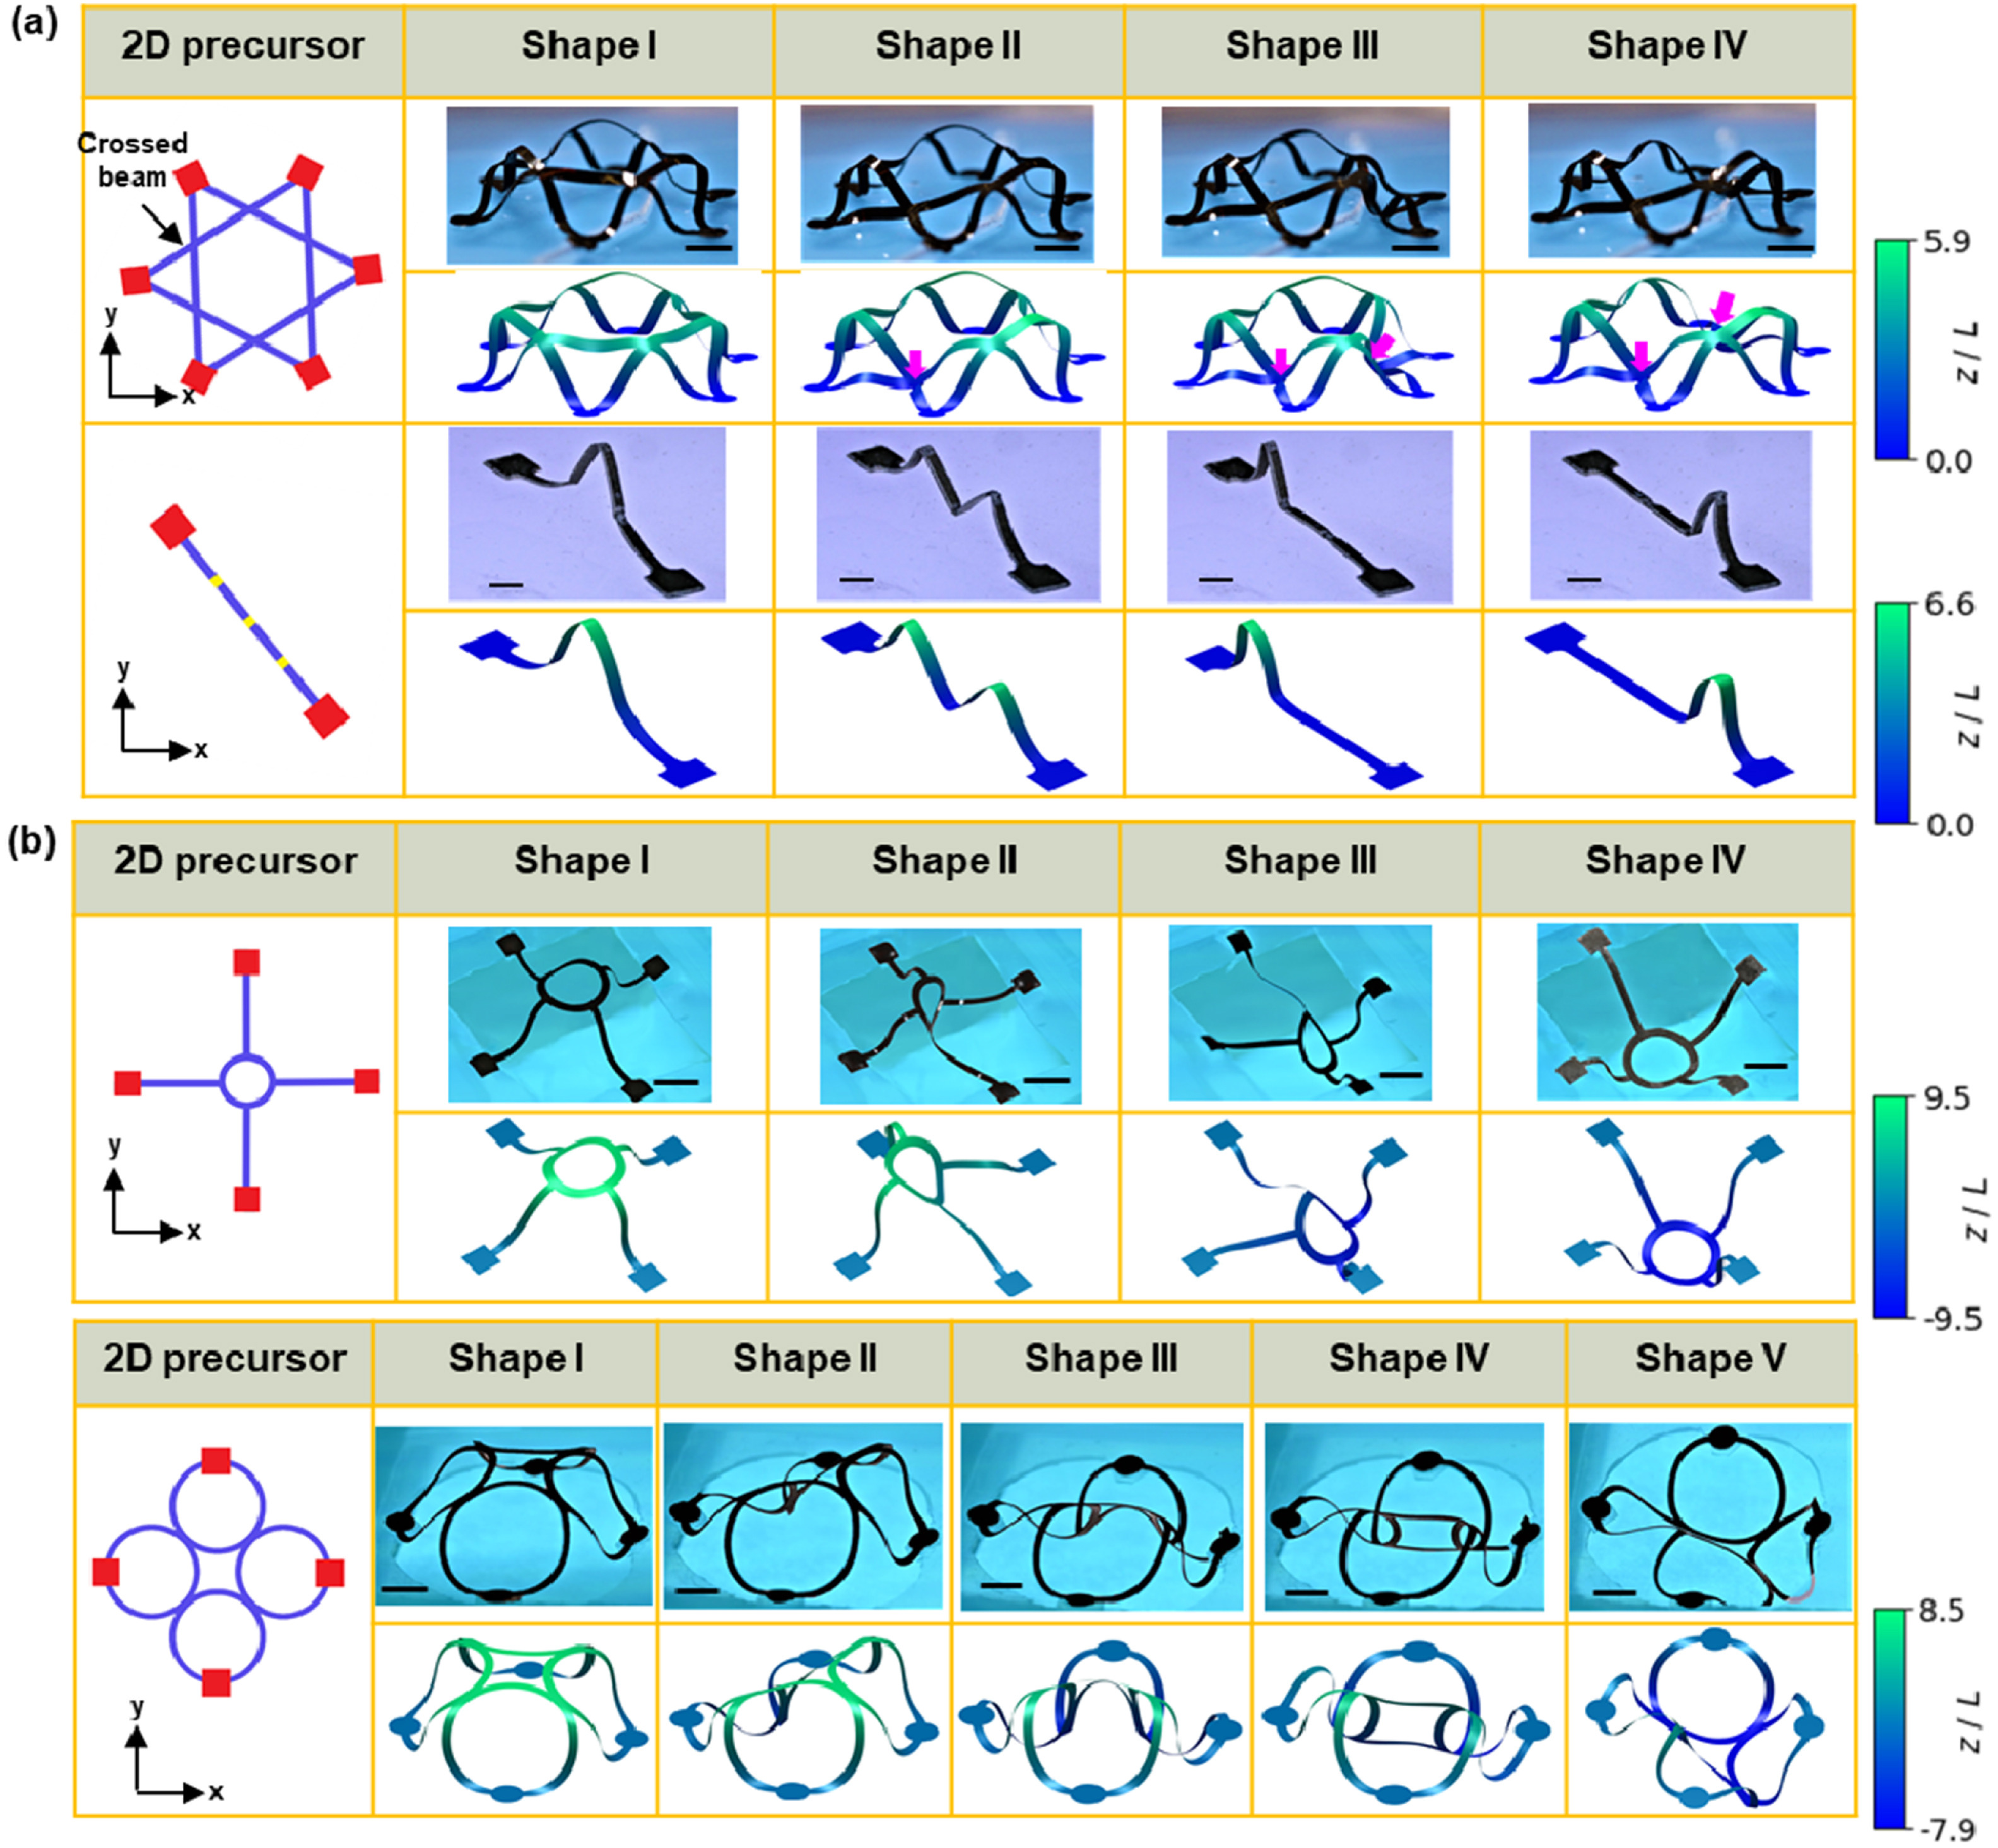
\includegraphics[width=\textwidth]{figure3.jpg}
  \caption{
    Diverse magnetically reconfigurable 3D structures.
    Optical images and computational modelling of multistable states for three types of structures:
    (a) 3D structures attached to a substrate.
        Pink arrows in the first structure indicate differences among the four shapes.
        Scale bars in the first and second structure are \SI{1}{\centi\meter} and \SI{2}{\milli\meter}, respectively.
    (b) 3D structures with the substrate underneath the structure removed.
        Scale bars, \SI{1}{\centi\meter}.
  }
  \label{fig:ms-3}
\end{figure}

\subsection{3D structures with diverse geometries}

The reconfiguration strategy and the energy landscape analysis described above are versatile and can be extended to different types of 3D structures in diverse geometries, as illustrated in \cref{fig:ms-3}.
\Cref{fig:ms-3}(a) shows an assembled ferromagnetic basket structure (shape I; film thickness: \SI{125}{\micro\meter}) and its multiple stable states (shapes II-IV) that can be achieved via magnetic control.
The pink arrows indicate differences among the four shapes.
In addition, by introducing creases to selective locations of a ribbon structure (crease thickness: \SI{70}{\micro\meter}; non-crease thickness: \SI{125}{\micro\meter}), we create a ferromagnetic origami structure, which is further tuned to display multiple stable configurations by using magnetic forces.

The elastomer substrate used for 3D assembly in \cref{fig:ms-1,fig:ms-2} provides essential support for the assembled 3D structures, but it also poses some limitations for the reconfiguration in the out of plane direction.
To allow more freedom for spatial reconfiguration, the substrate underneath the 3D table structure is removed, while the substrate adjacent to the bonding sites is maintained to support the 3D structure.
Such 3D structure on a hollow substrate allows bending up/down deformations across the plane of the substrate.
\Cref{fig:ms-3}(b) demonstrates a selection from a large variety of reconfigurable 3D structures on hollow substrates that have been investigated, including basket, single- and double-beam structures.

It is very interesting to note that the multistable configurations on hollow substates are sensitive to the orientation of the structures.
Take the table structure for example, when placed horizontally (i.e., the direction of gravity is perpendicular to the substrate), the structure only displays two stable states, buckled up and down.
However, when the table structure is placed vertically with the direction of gravity in the $x$ direction (\cref{fig:ms-3}(b)), in addition to the buckled up (Shape I) and down (Shape IV) states, it can deform into an asymmetric, twisted shape (Shape II), similar to state 3 of the table structure with an intact substrate.
This deformed shape can be further magnetically deformed into shape III, with the four bonding sites attached to the substrate and the rest of the structure self-supported in the air.

We also carry out energy landscape analysis for this structure, the details of which are presented in \cref{fig:ms-s6}.
Similar to the case with an intact substrate, we can distinguish several regimes with different numbers of stable states, depending on the three relevant energy scales: gravitational, stretching, and bending energies.

In addition, we quantitatively compare the dimensions of three representative 3D structures from experiments and modelling results and find negligible difference between them (\cref{tab:ms-comparison}), which further highlights the consistency between modelling and experimental results.

\begin{figure}[htb]
  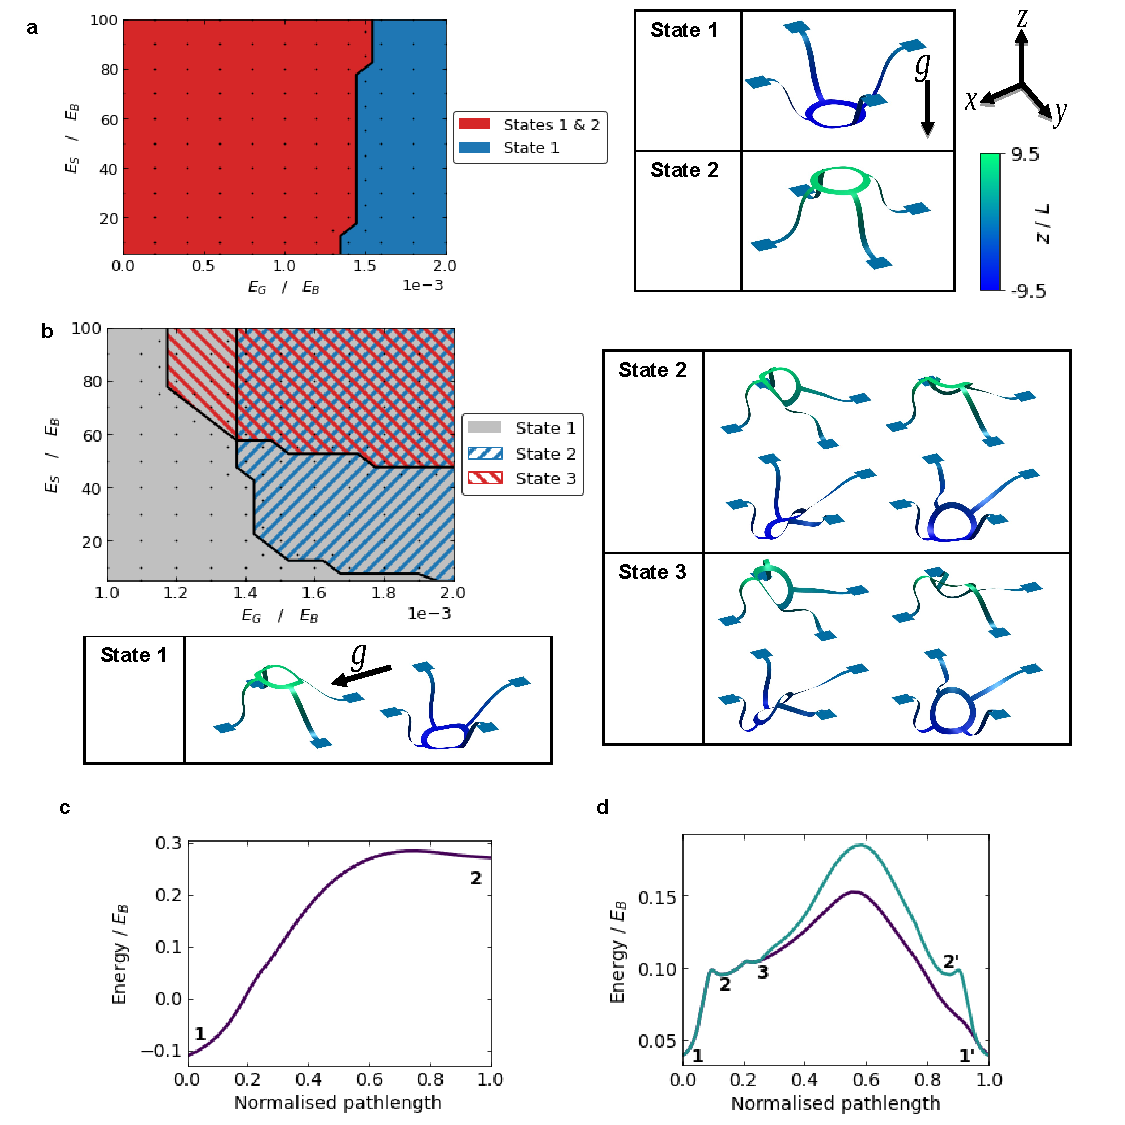
\includegraphics[width=\textwidth]{figureS6.pdf}
  \caption{
    (a-b) Phase diagrams of table structures on hollow substrates, with the direction of gravity in (a) the $z$-direction, (b) the $x$-direction.
          In panel (b), state I has two equivalent configurations, while both states II and III have four equivalent configurations.
    (c) Energy profile of the transition pathway from the buckled-down (state 1) to buckled-up (state 2) configurations when gravity is in the $z$-direction.
    (d) Energy profile of the transition pathway from the buckled-down (state 1) to buckled-up (state 1’) configurations when gravity is in the $x$-direction.
  }
  \label{fig:ms-s6}
\end{figure}

\begin{table}[htb]
  \setkeys{Gin}{width=\linewidth}
  \begin{tabularx}{\textwidth}{>{\centering}m{0.2\textwidth}CC >{\centering}m{0.2\textwidth}CC}
    \hline\hline
    \multicolumn{3}{c}{Experiment} & \multicolumn{3}{c}{Simulation} \\
    \cmidrule(lr){1-3}\cmidrule(lr){4-6}
    State & Width (mm) & Height (mm) & State & Width (mm) & Height (mm) \\
    \hline
    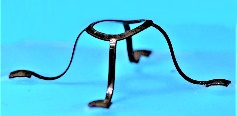
\includegraphics{comparison/experiment-1.png} & 32.2 & 9.2 &
    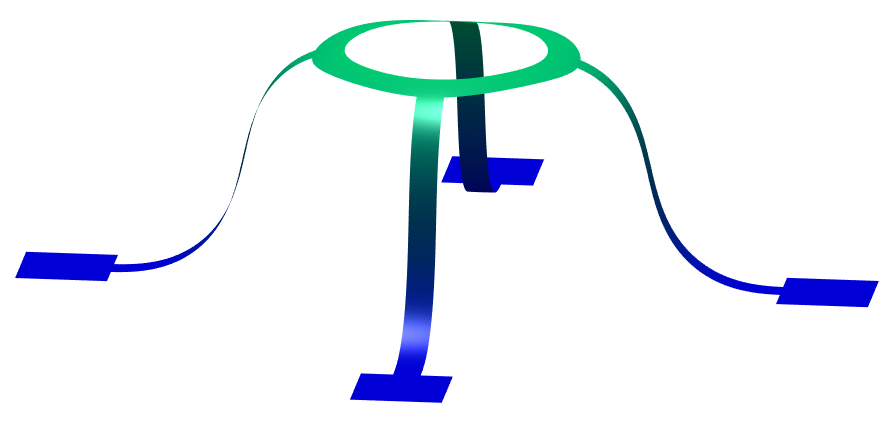
\includegraphics{comparison/simulation-1.png} & 33.5 & 9.0
    \\
    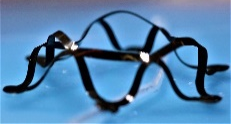
\includegraphics{comparison/experiment-2.png} & 37.6 & 10.7 &
    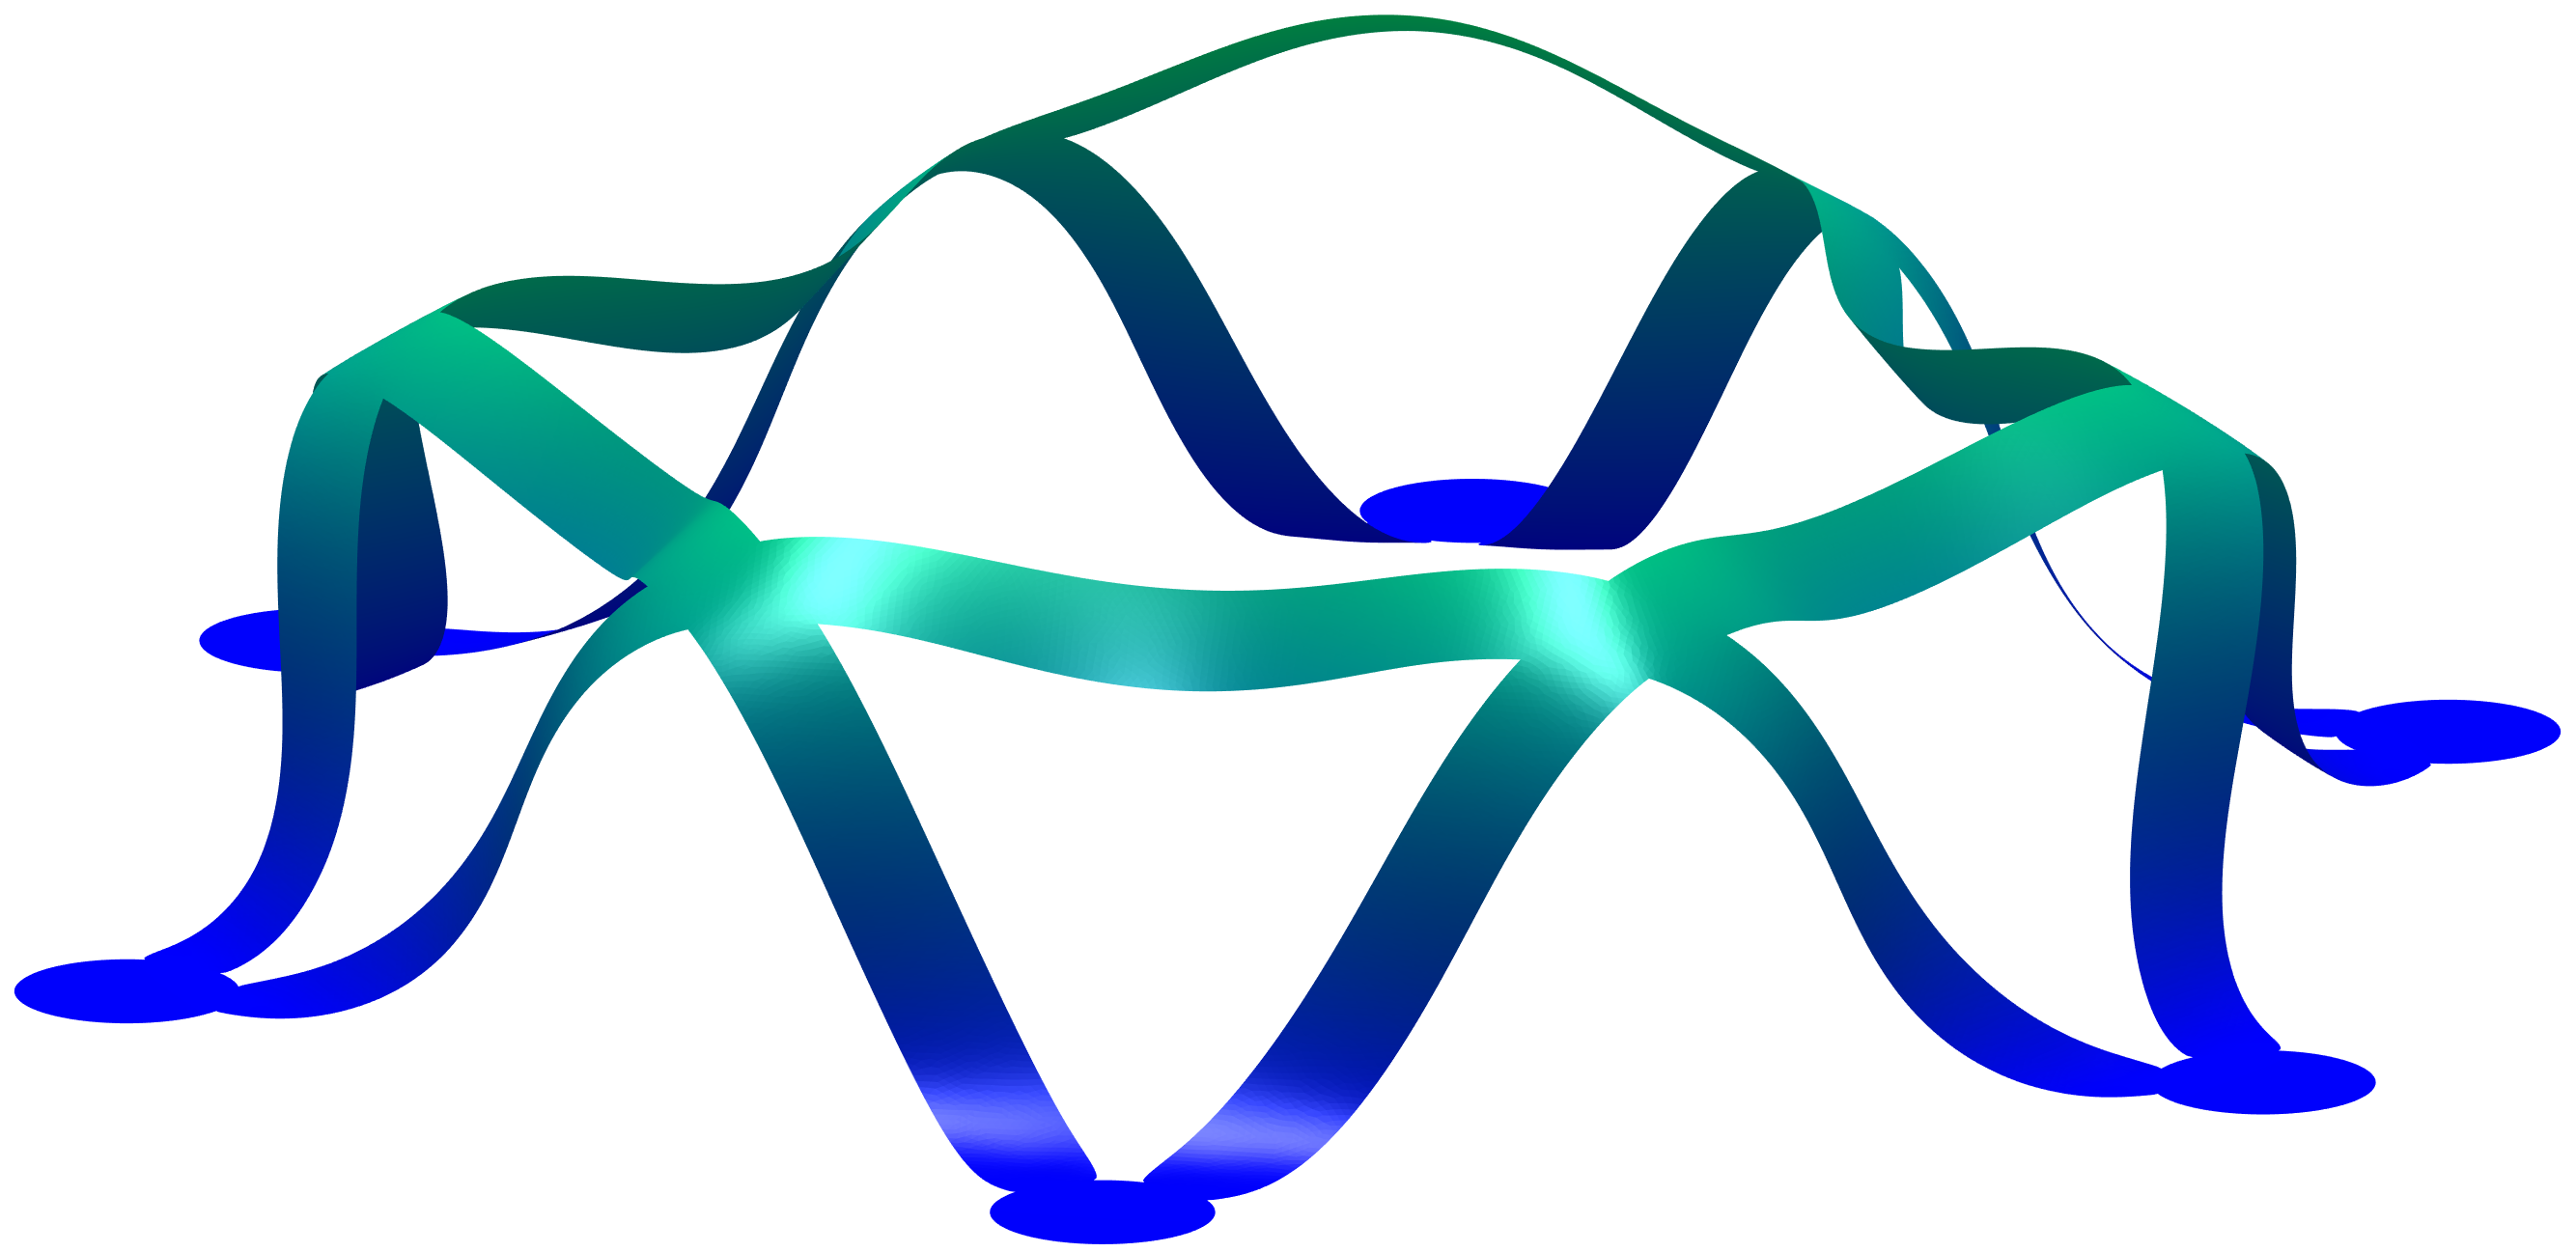
\includegraphics{comparison/simulation-2.png} & 38.0 & 10.9
    \\
    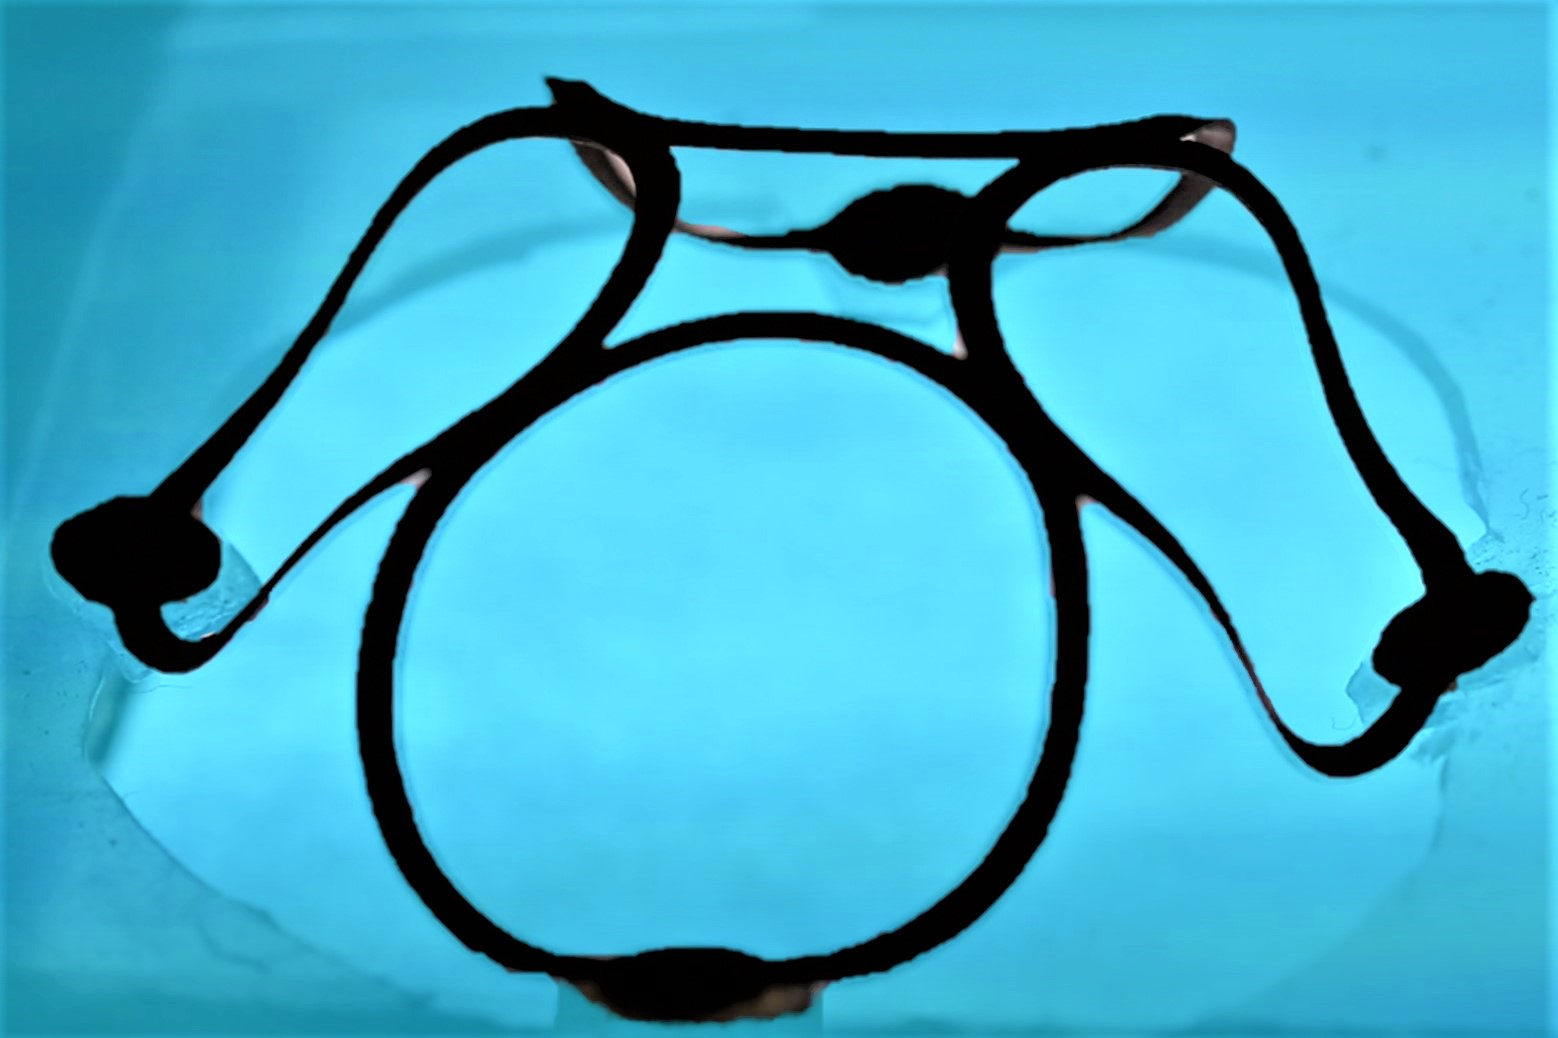
\includegraphics{comparison/experiment-3.png} & 31.5 & 10.1 &
    
\includegraphics{comparison/simulation-3.png} & 31.9 & 9.9
    \\
    \hline\hline
  \end{tabularx}
  \caption{The dimension comparison of experimental 3D structures and simulated 3D structures.}
  \label{tab:ms-comparison}
\end{table}


\subsection{Hybrid ferromagnetic structures}

In addition to tuning the strength and the direction of external magnetic forces for reconfiguration, an alternative and potentially more versatile means to realise magnetically controlled reconfiguration is through manipulating the distribution of magnetic materials within 3D hybrid structures.
\Cref{fig:ms-4}(a) schematically illustrates the fabrication process of such structures by locally integrating laser-cut ferromagnetic composite film patches (\SI{125}{\micro\meter} thick) onto a thin layer of inactive materials (PDMS, \SI{180}{\micro\meter} thick) and compressively buckling the 2D hybrid pattern into a 3D structure.

Following this strategy, reconfigurable 3D hybrid structures that resemble tables and flowers are fabricated and magnetically tuned to display five stable configurations (Shape I-V) using a portable magnet.
The deformed shapes can well maintain their configuration after the magnetic force is removed, the capability of which is the same as structures composed of a single layer of ferromagnetic composites.

In addition, 3D hybrid structures can potentially allow more local magnetic control by varying the direction and the strength of the residual magnetic field in each ferromagnetic patch through magnetization in different directions and mixing different concentrations of magnetic particles in the composite film, respectively.
This could be combined with information from the energy landscape analysis in order to design the patches so the deformation in a magnetic field most accurately follows the MEP.
However, this analysis and the exploration of other composition materials for reconfigurable 3D hybrid structures are beyond the scope of the current work.

\begin{figure}[htb]
  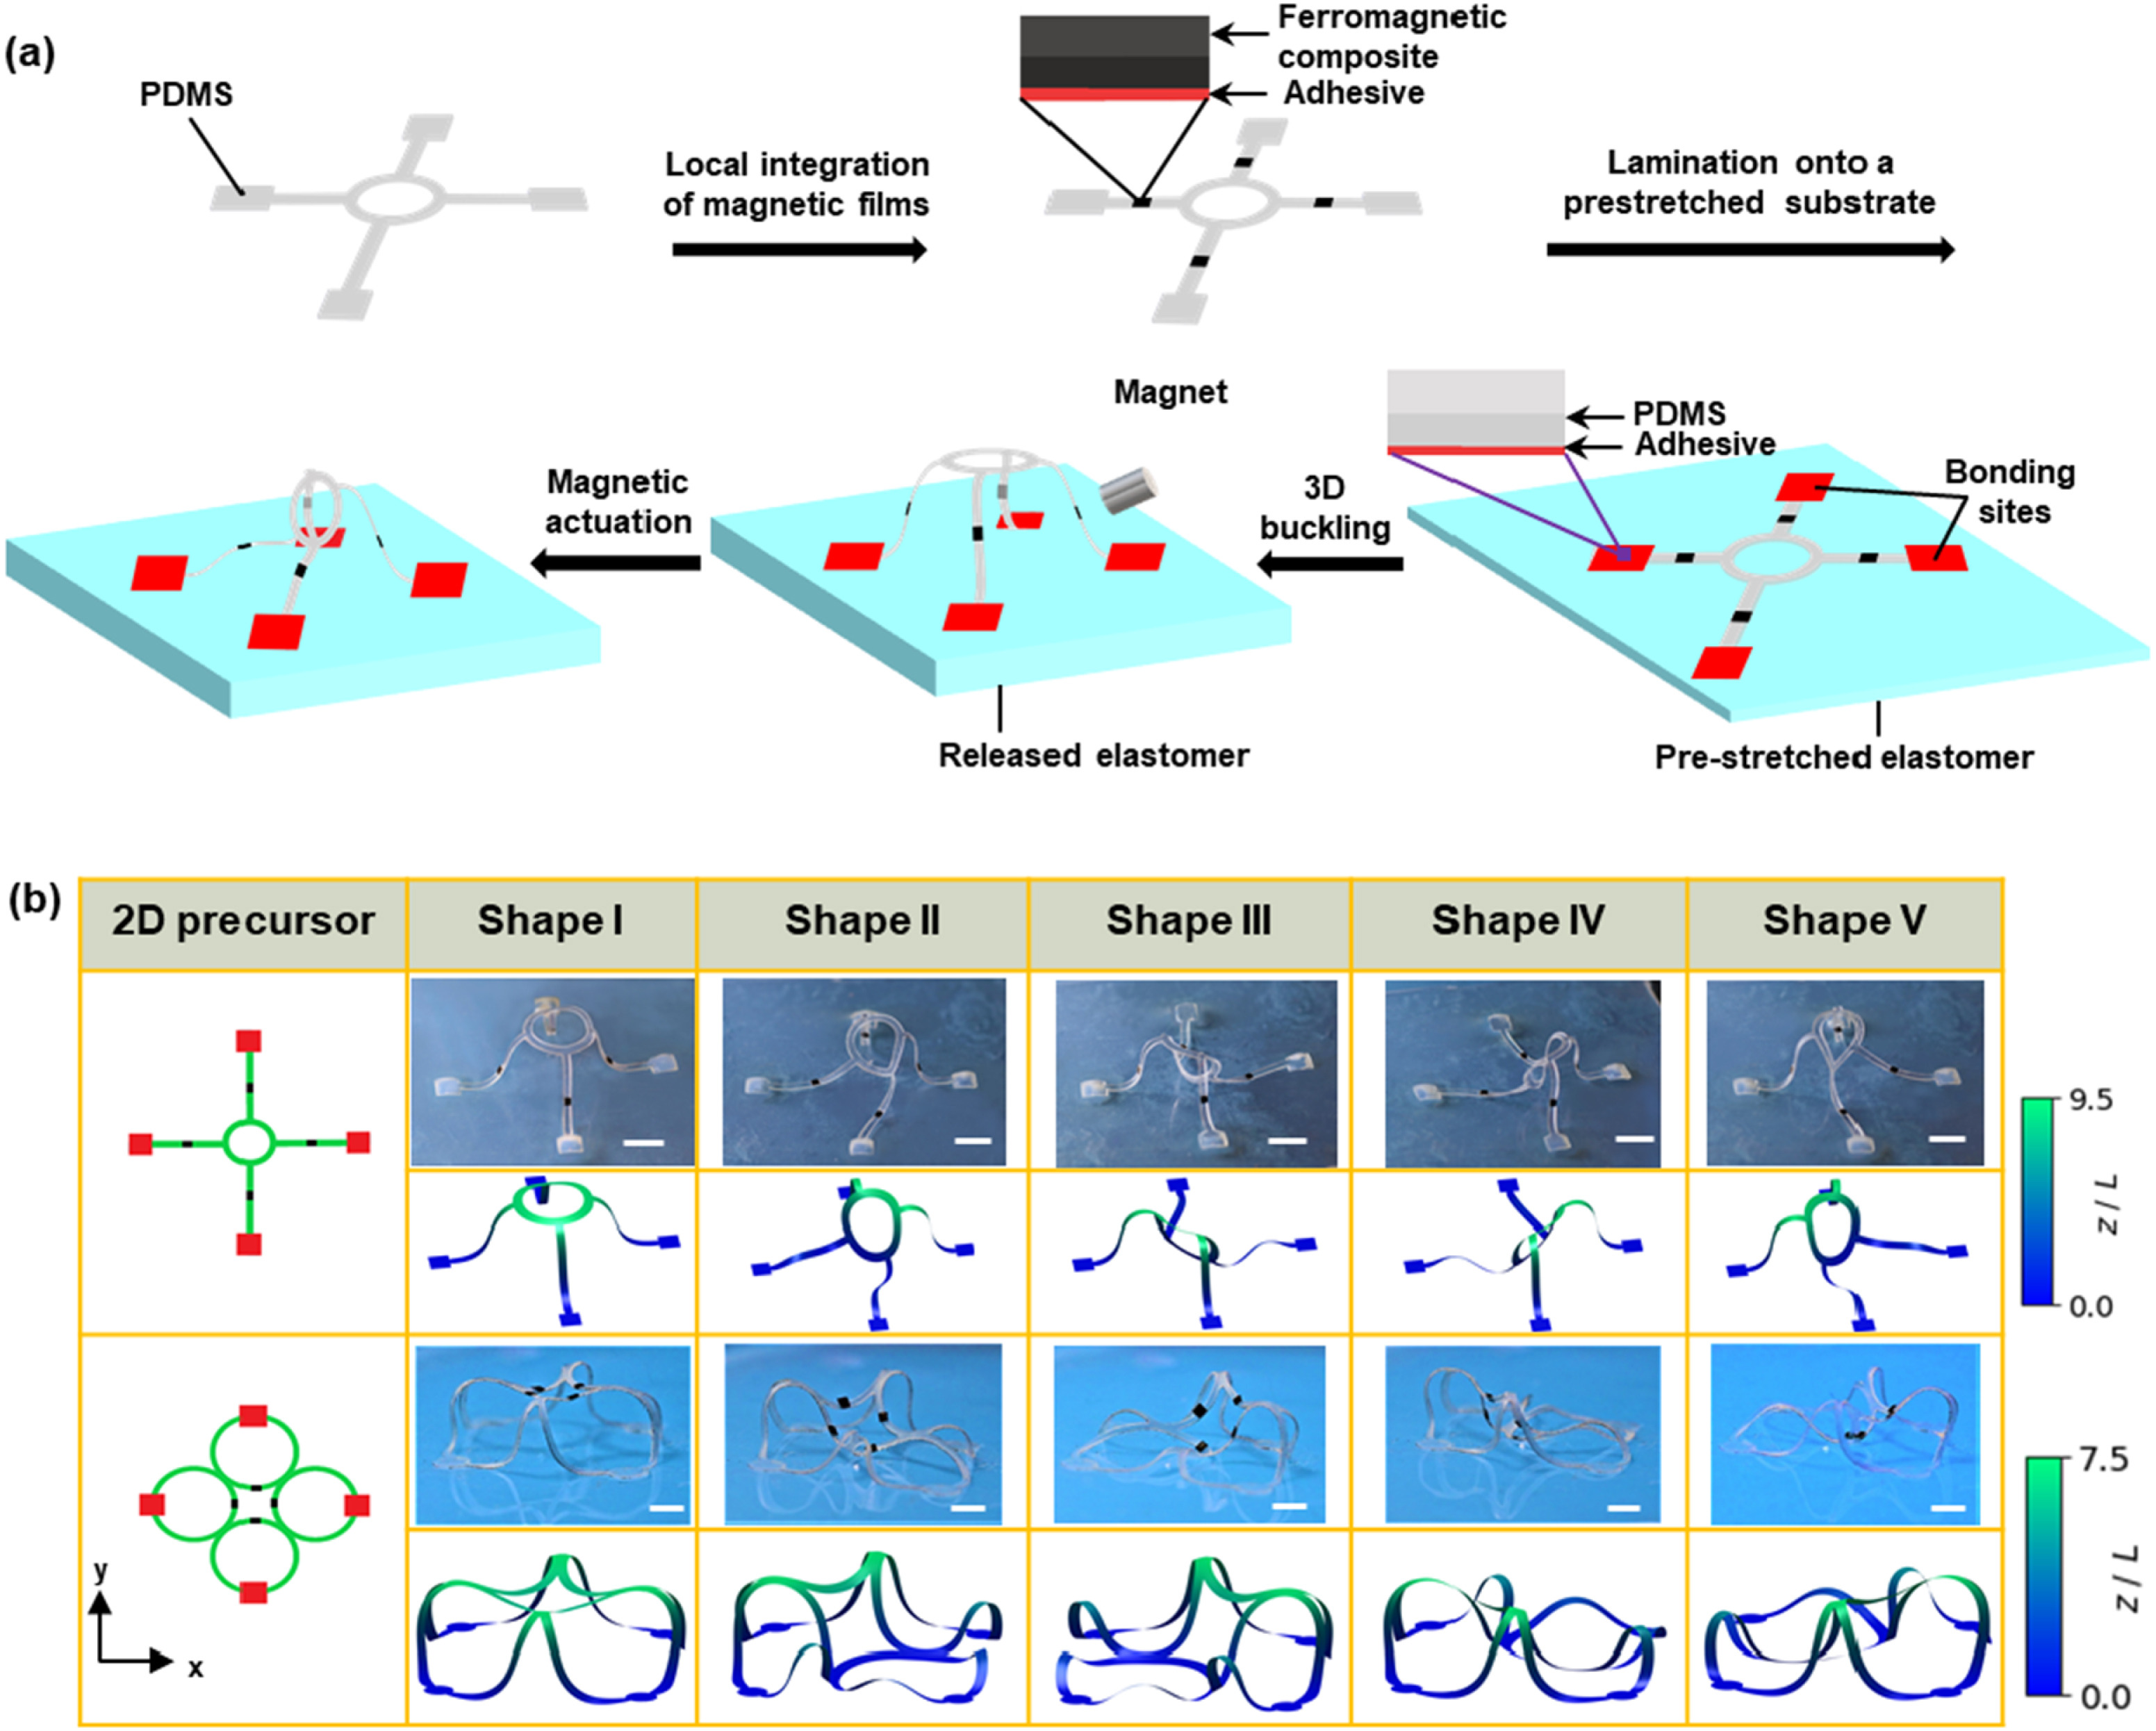
\includegraphics[width=\textwidth]{figure4.jpg}
  \caption{
    Locally tunable, heterogeneous 3D structures.
    (a) Schematic illustration of the fabrication process for locally controlled heterogeneous 3D ferromagnetic structures.
    (b) Optical images and computational modelling of multistable states for 3D structures composed of locally patterned ferromagnetic films on a thin layer of PDMS.
        Scale bars, \SI{1}{\centi\meter}.
  }
  \label{fig:ms-4}
\end{figure}


\subsection{Applications of reconfigurable 3D structures}
Using the techniques described above, our experimental collaborators have designed two proof-of-principle applications that demonstrate the potential offered by reconfigurable ferromagnetic mesostructures.

Firstly, functional materials and components may be integrated onto the 2D precursor, providing access to tunable 3D functional devices.
This is demonstrated using a reconfigurable light emitting system in \cref{fig:ms-5}(a).
Here, two light emitting diodes (LEDs) are integrated onto designated locations of a double-beam structure with copper thin films connected to the LED serving as contacts for LED activation.
The cross-links in the structure can be individually buckled using magnetic actuation, deforming the structure from shape I to II (or III).
This enables a firm contact between the LED on the structure with the copper contacts on the substrate, connecting to an external power supply and activating the LED.
The multistability of the structure then enables the LED to maintain its “on” status after the magnetic force is removed.
When the two beams are simultaneously deformed to form stable configuration IV using a magnet, both LEDs are turned on.
This simple example suggests a broad range of possibilities in other types of electronic and optoelectronic devices.

\begin{figure}[htb]
  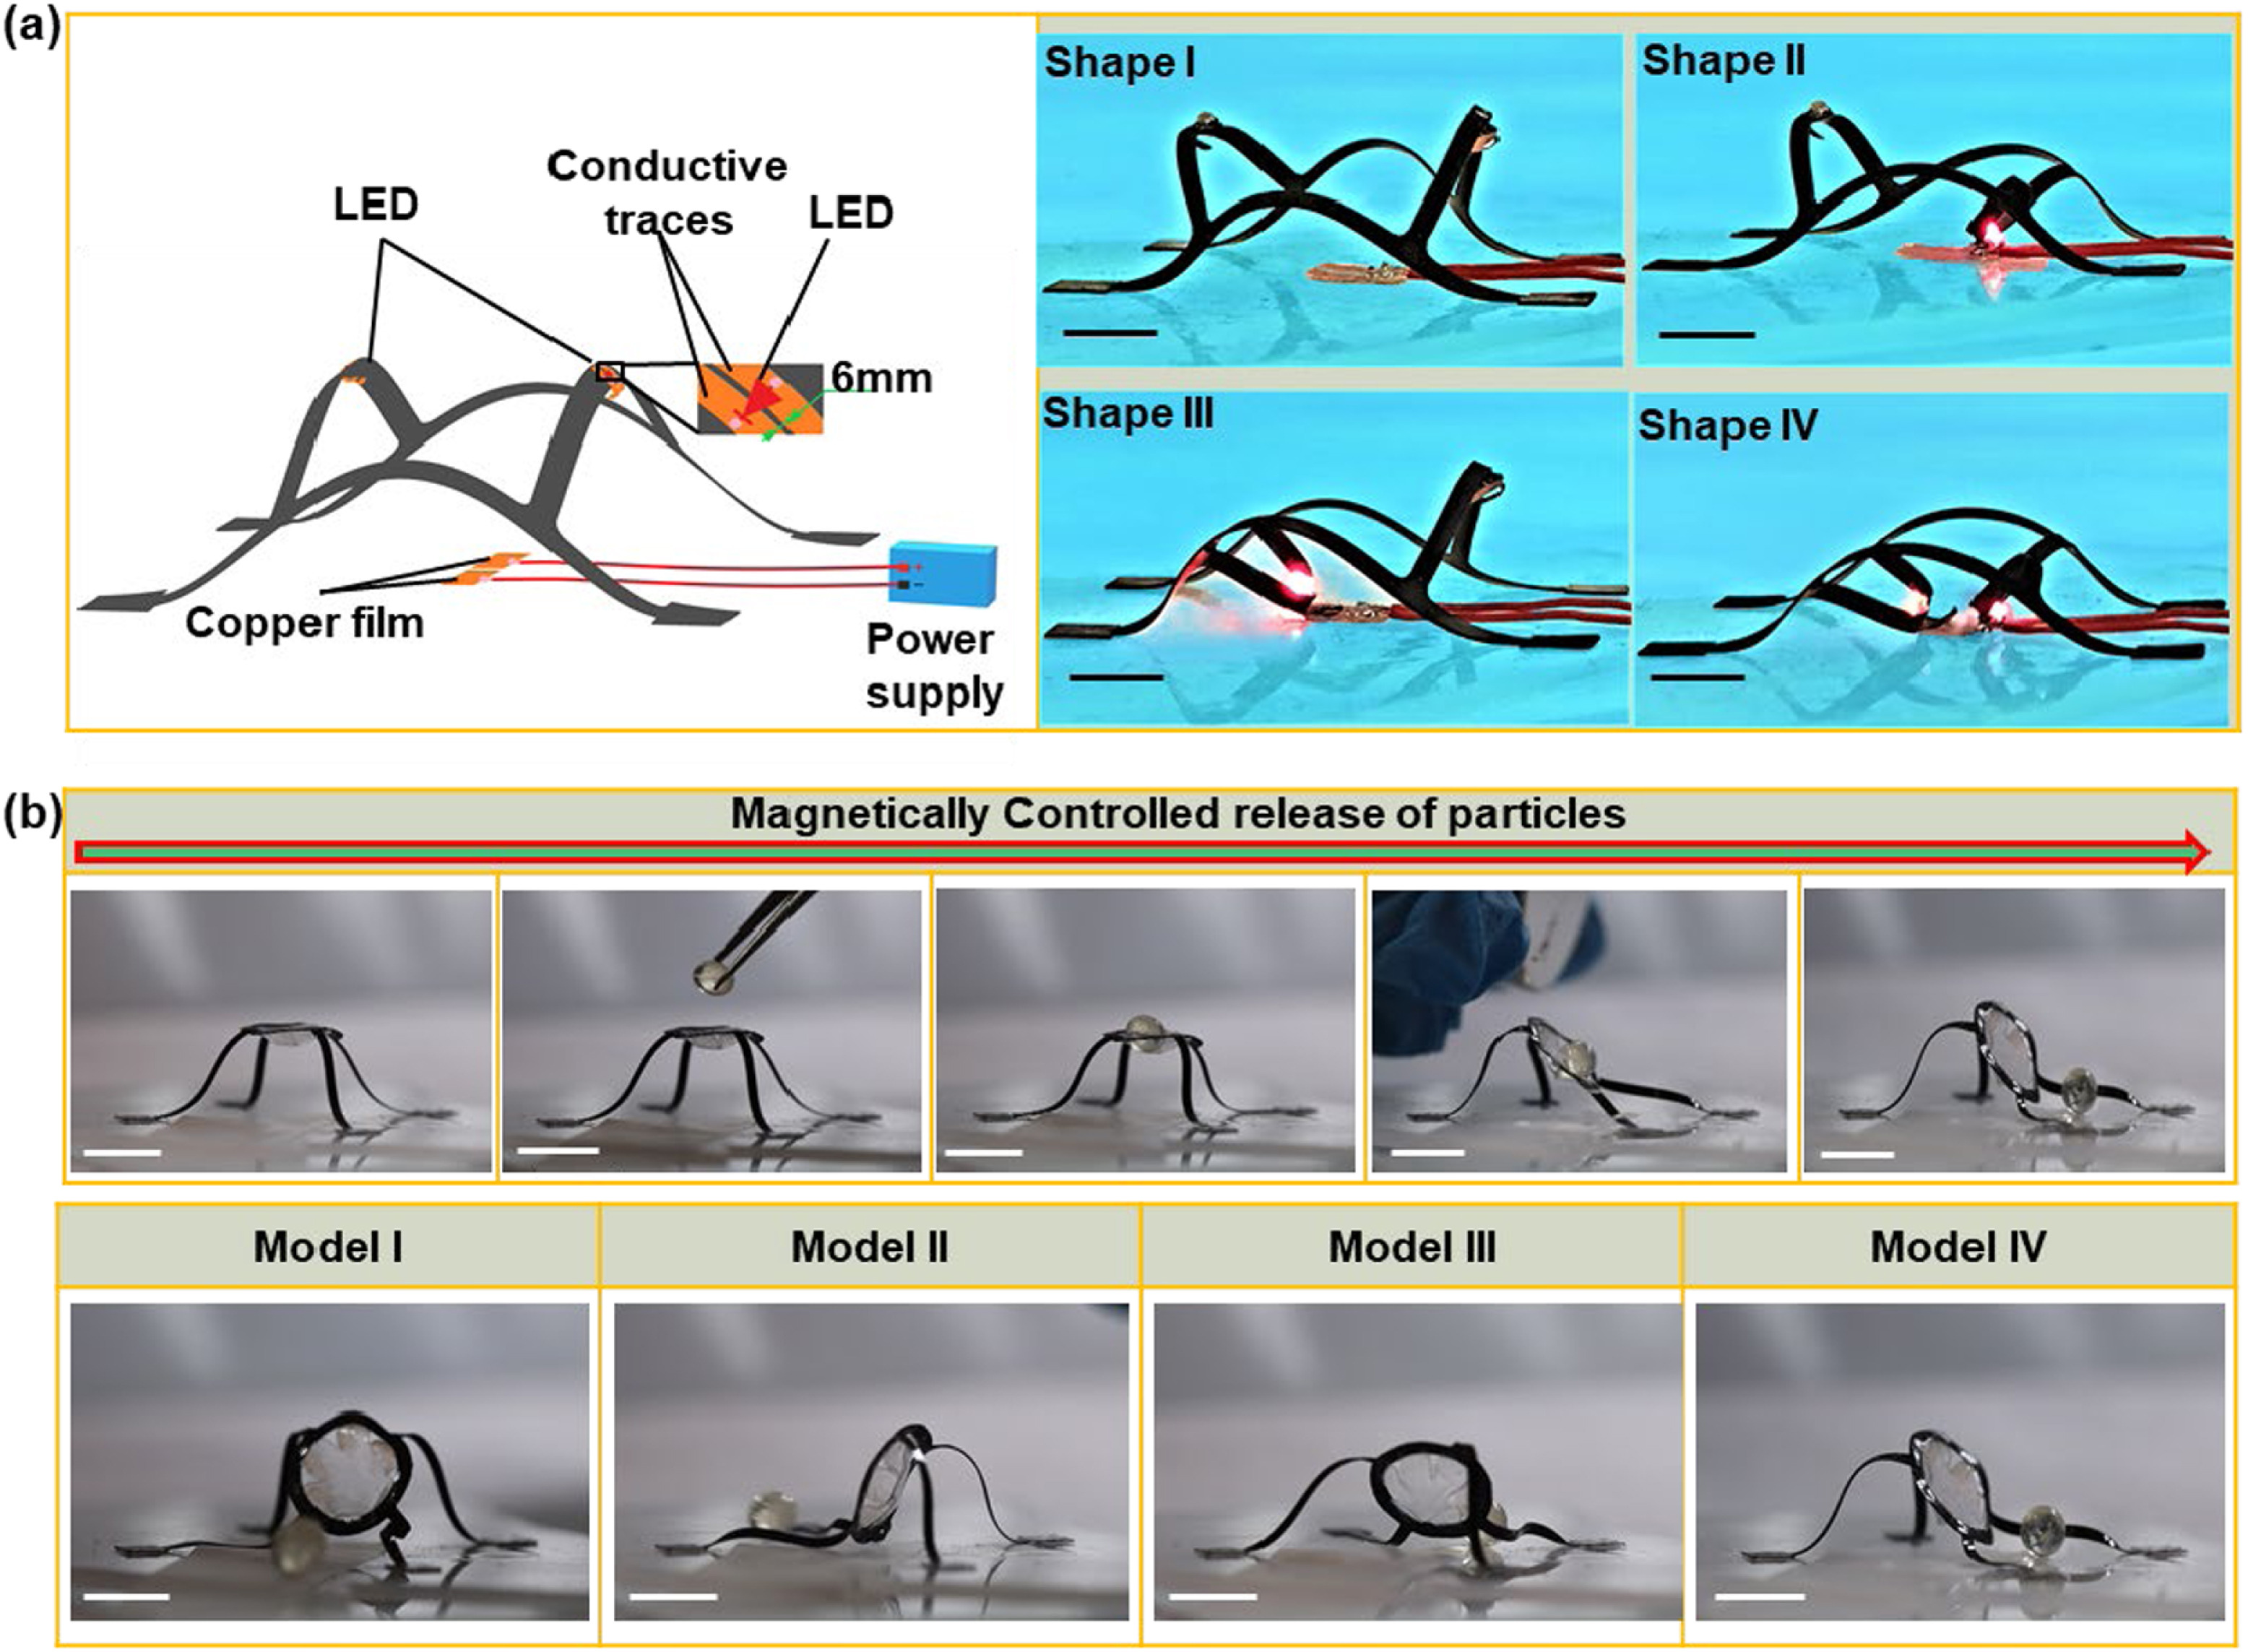
\includegraphics[width=\textwidth]{figure5.jpg}
  \caption{
    Applications of reconfigurable structures in on-demand 3D light emitting systems and controlled particle delivery.
    (a) Schematic illustration and optical images of a 3D light emitting system that can be reconfigured among its multistable states to switch the LEDs on and off.
    (b) Controlled release of particles in four different directions (Modes I-IV) enabled by four possible stable states of the table structure.
    Scale bars, \SI{1}{\centi\meter}.
  }
  \label{fig:ms-5}
\end{figure}

Based upon our investigations of the 3D table structure, a device is created for the delivery of particles in a well-controlled manner.
As shown in \cref{fig:ms-5}(b), a thin layer of pure PDMS film is placed in a concave shape in the centre of the table, in order to support a silica particle.
This film that supports the particle is insensitive to the applied magnetic field when the table structure is magnetically actuated, thereby exerting minimal influence on the reconfiguration of the whole structure.
The table structure itself is designed to be in the 2 state region of the phase diagram, \cref{fig:ms-1}(c), such that it exhibits one upright state and a second state in four different orientations (modes I-IV).
To trigger the delivery of the particle, a portable magnet is used to manipulate the structure into one of these different orientations, leading to well-controlled particle delivery in a chosen direction.
Therefore, such flexible, remotely reconfigurable structures could have a lot of potential applications in controlled delivery.



\section{Discussion}

To conclude, we have tightly integrated experiments and modelling to survey the energy landscapes of highly nonlinear 3D ferromagnetic structures for the development of reconfigurable systems.
Our systematic computational analysis predicts a design phase diagram for a targeted number of stable states by varying essential material properties and geometries.
It also allows us to systematically identify highly complex transition paths among the distinct stable states that minimise the energy barriers, without the need to prescribe an expected pathway for structural transformations a priori.
These predictions are thoroughly validated by our experiments of creating multistable 3D ferromagnetic structures and magnetically reconfiguring the structures among their multistable states following different pathways rapidly, in a remote, on-demand manner.

Using this strategy, a plethora of symmetric and asymmetric 3D mesostructures of diverse geometries are realised and reconfigured among their multistable states, including those that resemble ribbons, tables, baskets, flowers, boxes, single and double beams.
These versatile reconfigurable structures have a range of possible applications, illustrated by the integration of electronic components to create reconfigurable light-emitting functional devices, and a magnetically actuated table structure for particle delivery.

We believe our fundamental studies on the reconfigurational behaviours of 3D structures establish the foundations for a robust and reproducible modelling approach that may be applied more broadly to the design and development of diverse types of reconfigurable structures and systems.
This may include origami, kirigami and stimuli-responsive structures beyond magnetic actuation, where the exploration of energy landscapes could aid in understanding the reconfiguration and the tunability of multistable states.

It is also interesting to explore the integration of functional materials with locally patterned magnetic films of different magnetization directions \cite{Kim2018,Alapan2020}, and stiffness manipulation \cite{Zhai2020} to expand the design space of possible hybrid structures and to potentially enable multi-stimuli-responsive structures and soft machines.
We believe these studies will provide important insights for the design of reconfigurable structures and functional systems for wide-ranging applications, such as in deployable solar panels, phononics, morphable architected materials, and soft robotics.

\begin{table}[]
  \begin{tabularx}{\textwidth}{>{\hsize=.3\hsize\linewidth=\hsize}C >{\hsize=.55\hsize\linewidth=\hsize}C >{\hsize=2.1\hsize\linewidth=\hsize}C >{\hsize=1.05\hsize\linewidth=\hsize}C}
    \hline\hline
    Topic & Symbol & Parameter description & Value \\
    \hline
    \multirow{9}{*}{\rotatebox[origin=c]{90}{Structure}}
          & $L$            & Arm width              & 1.04 / 0.8 / \SI{0.5}{\milli\metre} \\
          & ---            & Arm length             & $12.5 L$ \\
          & $r_\text{out}$ & Outer ring radius      & $5 L$ \\
          & $r_\text{in}$  & Inner ring radius      & $3.75 L$ \\
          & ---            & Mesh resolution        & $0.1 L$ \\
          & $t$            & Thickness              & \SI{150}{\micro\metre} \\
          & $\rho$         & Density                & \SI{2.59}{\gram\per\centi\meter\cubed} \\
          & $Y$            & Young's modulus        & \SI{1.4}{\mega\pascal} \\
          & $\nu$          & Poisson ratio          & 0.3 \\
          & ---            & Compressive strain     & 0.3 \\
    \hline
    \multirow{4}{*}{\rotatebox[origin=c]{90}{L-BFGS}}
          & $m$      & Iteration memory             & 10 \\
          & ---      & Initialisation iterations    & \num{10000} \\
          & ---      & Initialisation force density & \SI{10}{\newton\per\meter\squared} \\
          & ---      & Gradient RMS convergence     & $10^{-10}$ \\
    \hline
    \multirow{6}{*}{\rotatebox[origin=c]{90}{Pathways}}
          & $\alpha$ & BITSS energy constraint strength    & 10 \\
          & $\beta$  & BITSS distance constraint error     & 0.1 \\
          & $f$      & BITSS distance reduction factor     & 0.5 \\    
          & ---      & BITSS coefficient regularity        & 100 iterations \\    
          & ---      & String reparametrisation regularity & 300 iterations \\
          & ---      & String number of images             & 20 \\
    \hline\hline
  \end{tabularx}
  \caption{\label{tab:ms-params}
    Values of the parameters that are used throughout this chapter, unless otherwise specified.
  }
\end{table}
